\documentclass[a4paper,leqno,nobib,sfsidenotes]{tufte-book}


%% Paquetes relacionados con el lenguaje y la localización del texto
\usepackage[utf8]{inputenc}
\usepackage[T1]{fontenc}
\usepackage[spanish,es-tabla]{babel}
\usepackage{csquotes}   %% Comillas dobles
\decimalpoint           %% Usar punto decimal en lugar de una coma
\usepackage[
  backend=biber,
  autocite=footnote,    %% Inserta las ref. en el margen con \autocite
  style=authoryear,     %% Orden en que aparece la info. en la bibliografía
  uniquename=init,      %% Usa iniciales para distinguir apellidos repetidos
  maxcitenames=2,       %% Se citan a lo más dos autores
  mincitenames=1,
  doi=false,            %% Ignora estos campos del archivo .bib
  isbn=false,
  url=false,
  eprint=false,
  dashed=false
]{biblatex}


%% Paquetes relacionados con tablas, figuras y otras gráficas
\usepackage{float}      %% Para gráficos flotantes en la página
\usepackage{booktabs}   %% Para tablas más sofisticadas
\usepackage{multirow}   %% Para columnas y renglones extendidos en tablas
\usepackage{graphicx}   %% Para gráficos generales


%% Paquetes relacionados con el formato de ciertas secciones del texto
\usepackage{caption}    %% Para el texto debajo de gráficos flotantes
\usepackage{multicol}   %% Para secciones con texto dividido en columnas
\usepackage{enumitem}   %% Para listas con viñetas
\setlist[itemize]{label=\textbullet}


%% Paquetes relacionados con los ambientes matemáticos
\usepackage{amsmath}
\usepackage{amsthm}
\usepackage{amssymb}

%% Definición de los ambientes matemáticos
\providecommand{\casename}{Caso}
\providecommand{\definitionname}{Definición}
\providecommand{\examplename}{Ejemplo}
\providecommand{\propositionname}{Proposición}
\providecommand{\theoremname}{Teorema}
\providecommand{\lemmaname}{Lema}
\providecommand{\corollaryname}{Corolario}
\providecommand{\remarkname}{Escolio}
\theoremstyle{definition}
\newtheorem{defn}{\protect\definitionname}
\newtheorem{expl}{\protect\examplename}
\theoremstyle{plain}
\newtheorem{prop}{\protect\propositionname}
\newtheorem{thm}{\protect\theoremname}
\newtheorem{lem}{\protect\lemmaname}
\newtheorem{cor}{\protect\corollaryname}
\theoremstyle{remark}
\newtheorem{rem}{\protect\remarkname}

%% Configuración del enumerado de los ambientes matemáticos
\newlist{casenv}{enumerate}{4}
\setlist[casenv]{leftmargin=*,align=left,widest={iiii}}
\setlist[casenv,1]{label={{\itshape\ \casename} \arabic*.},ref=\arabic*}
\setlist[casenv,2]{label={{\itshape\ \casename} \roman*.},ref=\roman*}
\setlist[casenv,3]{label={{\itshape\ \casename\ \alph*.}},ref=\alph*}
\setlist[casenv,4]{label={{\itshape\ \casename} \arabic*.},ref=\arabic*}

%% Símbolo para indicar el final de un ejemplo
\newcommand\xqed[1]{\leavevmode\unskip\penalty9999 \hbox{}\nobreak\hfill\quad\hbox{#1}}
\newcommand\exend{\xqed{\(\blacklozenge\)}}


%% Configuración para colocar automáticamente hipervínculos en el PDF
\PassOptionsToPackage{
  unicode=true,
  pdfusetitle,
  bookmarks=true,
  bookmarksnumbered=true,
  bookmarksopen=false,
  breaklinks=false,
  pdfborder={0 0 1},
  backref=false,
  colorlinks=false
}{hyperref}


%% Configuración para escribir pseudocódigo
\usepackage[vlined,linesnumbered,ruled]{algorithm2e}
\setkeys{Gin}{width=\linewidth,totalheight=\textheight,keepaspectratio}

\SetKw{Error}{error}
\SetKw{And}{and}
\SetKw{Or}{or}
\SetKw{Not}{not}
\SetKw{True}{true}
\SetKw{False}{false}
\SetKw{Nil}{nil}
\SetKw{Down}{down to}
\SetCommentSty{textit}
\SetKwComment{Comment}{$\triangleright$ }{}
\SetFuncSty{textsc}
\DontPrintSemicolon
\SetAlgorithmName{Pseudocódigo}{}


%% Se eliminan algunos campos innecesarios de las ref. bibliográficas
\makeatletter
\AtBeginDocument{
  \AtEveryBibitem{\clearfield{month}}
  \AtEveryBibitem{\clearfield{day}}
  \AtEveryBibitem{\clearfield{note}}
  \AtEveryBibitem{\clearlist{location}}
  \AtEveryBibitem{\clearfield{eventtitle}}
  \DeclareFieldFormat[article,inbook,incollection,inproceedings,patent,thesis,unpublished]{citetitle}{#1}
  \DeclareFieldFormat[article,inbook,incollection,inproceedings,patent,thesis,unpublished]{title}{#1} 
}
\makeatother


\title{Análisis de Algoritmos}
\author{Carlos A. Oliva Moreno}
\addbibresource{referencias.bib}

\begin{document}
  \maketitle
  
  \tableofcontents{}
  
  \chapter{Conceptos fundamentales}

Un \textbf{problema computacional} es una relación entre dos valores o conjuntos de valores: uno de \textbf{entrada} y otro de \textbf{salida}. 
Por ej., el problema de \textsc{Ordenamiento} se define formalmente de la sig. manera:
\begin{itemize}
  \item \emph{Entrada}: una secuencia de \(n\in\mathbb{N}\) elementos comparables, \(A=\{a_1,a_2,\dots,a_n\}\).
  \item \emph{Salida}: una permutación de la secuencia de entrada, \(A'=\{a'_1,a'_2,\dots,a'_n\}\), tal que \(a'_1\leq a'_2\leq\dots\leq a'_n\).
\end{itemize}
Un \textbf{caso específico} para un problema computacional determinado es cualquier valor o conjunto de valores que satisfacen la descripción de la entrada del problema.
Por ej., dos casos específicos para el problema de \textsc{Ordenamiento} son las secuencias \(\{4,7,5,1\}\) y \(\{d,x,j,e\}\).

Un \textbf{algoritmo} es un procedimiento inambiguo para transformar la entrada de un problema computacional determinado a la salida correspondiente.
Un algoritmo es \textbf{correcto} si y solo si, para todo caso específico, el algoritmo termina su ejecución y produce un resultado que cumple la descripción de la salida del problema.
Un algoritmo \textbf{resuelve} el problema en cuestión si y solo si es correcto.

Una \textbf{estructura de datos} es una colección de reglas y procedimientos para organizar, accesar y manipular un conjunto de datos.

Por último, el \textbf{análisis de algoritmos} es la colección de técnicas y herramientas matemáticas que se usan para caracterizar las propiedades particulares de un algoritmo determinado de forma independiente a su implementación en hardware y/o software. 
El análisis de un algoritmo consiste en determinar al menos dos características:
\begin{itemize}
  \item La \textbf{corrección}: ¿el algoritmo es correcto?
  \item La \textbf{eficiencia}: ¿cuál es el \emph{orden de crecimiento} del 
  tiempo de ejecución del algoritmo con respecto al tamaño de la entrada?
\end{itemize}
Un algoritmo es \textbf{eficiente} si y solo si el orden de crecimiento
de su tiempo de ejecución es polinomial.
Casi todo problema computacional puede resolverse por medio de un algoritmo de fuerza bruta.
Es por esto que el objetivo es diseñar algoritmos que no solo sean correctos, sino que también sean lo más eficientes posible.
\marginnote[-15\baselineskip]{%
  Dependiendo de la aplicación y tipo del algoritmo que se está analizando, hay otras características que también podrían ser de interés determinar de dicho algoritmo.
  Por ej., una característica frecuentemente estudiada es el orden de crecimiento de la cantidad de memoria ocupada por el algoritmo con respecto al tamaño de la entrada.
}

\marginnote[-2\baselineskip]{\textbf{Literatura consultada}: \textcite{cormen_introduction_2009}, pp. 5-14 y 20-22; \textcite{skiena_algorithm_2012}, pp. 3-13.}

  \chapter{Análisis de la corrección de un algoritmo}

El primer paso al analizar un algoritmo es determinar si este es correcto o incorrecto. 
El procedimiento que se sigue para llevar a cabo esta tarea se denomina \textbf{análisis de la corrección de un algoritmo}.

\section{El contraejemplo}

\marginnote[0.5\baselineskip]{Se recomienda buscar un contraejemplo para un algoritmo antes de hacer la demostración de su corrección.}

\marginnote[1.5\baselineskip]{Si no se encuentra un contraejemplo para un algoritmo determinado, esto no implica que dicho algoritmo es correcto.}

\marginnote[1.5\baselineskip]{La demostración de la corrección de un algoritmo debe explicar no solo por qué el algoritmo es correcto, sino también por qué no es incorrecto.}

Para demostrar que un algoritmo determinado es incorrecto, basta con producir un \textbf{contraejemplo}; esto es, un caso específico para el cual el algoritmo no termina su ejecución o no produce un resultado que cumple las características de salida del problema. 
Para encontrar un contraejemplo, se recomienda experimentar primero con los casos específicos más complicados para el algoritmo; p. ej., aquellos que contengan valores empatados o que mezclen valores de frontera de extremos opuestos. 
El contraejemplo debe ser lo más simple y pequeño posible; idealmente la razón de por qué el algoritmo es incorrecto debe ser inmediatamente clara. 
Así, una vez encontrado un contraejemplo, se recomienda simplificarlo tanto como sea posible y presentarlo junto con el resultado incorrecto que produjo el algoritmo y el resultado correcto que debió producir.

\section{La invariante de lazo}

\marginnote[0.5\baselineskip]{%
  La diferencia entre la invariante de lazo e inducción es que el primer método es una aplicación especializada del segundo.
}

Una \textbf{invariante de lazo} es una proposición lógica que se cumple inmediatamente antes de cada iteración y al finalizar la ejecución de un bucle determinado.
La invariante se define en función de cada iteración \(i\).
Demostrar que una invariante de lazo se cumple para todas las iteraciones es un procedimiento análogo a una demostración por inducción y consta de los sig. pasos: 
\begin{enumerate}
  \item \textbf{Inicialización}: se determina el estado en que se encuentra el algoritmo antes de ejecutar la primera iteración y se demuestra que la invariante se cumple bajo estas condiciones.
  \item \textbf{Mantenimiento}: se supone que la invariante se cumple antes de comenzar alguna iteración arbitraria \(j\) y se determina el estado en que se encuentra el algoritmo como consecuencia de ello. 
  Después, se ejecuta la iteración \(j\) y se demuestra que la invariante se cumple antes de comenzar la iteración \(j+1\).
  \item \textbf{Finalización}: se determina cuál es el estado del algoritmo al salir del bucle y se utiliza junto con la invariante para demostrar que el algoritmo es correcto o para caracterizar alguna propiedad particular del mismo. 
\end{enumerate}

\marginnote[-3.5\baselineskip]{%
  Estrictamente hablando, en la finalización se debería demostrar que la invariante se sigue cumpliendo cuando la condición de paro del bucle es falsa.
  Sin embargo, obsérvese que en el mantenimiento se demuestra no solo que la invariante se cumple inmediatamente antes de cada iteración, sino que también se sigue cumpliendo inmediatamente \emph{después} de cada iteración, incluyendo la \emph{última}.
  Es por eso que en la finalización se puede suponer que la invariante se sigue cumpliendo al terminar la ejecución del bucle.
}

\section{Recomendaciones para el diseño de algoritmos correctos}

\paragraph*{Definir la salida del problema correctamente.}{%
  Las características de salida no deben ser ambiguas y deben describir cómo determinar de forma inequívoca si el resultado es correcto.
  Tampoco deben constar de objetivos compuestos, esto es, de múltiples objetivos que deben alcanzarse al mismo tiempo.
}

\paragraph*{Típicamente, entre más restrictivas sean las características de entrada, menor es la dificultad para resolver el problema.}{
  Se recomienda comenzar por diseñar un algoritmo correcto que admita entradas con características muy particulares y después extenderlo a entradas más generales. 
}

\paragraph*{Analizar la complejidad computacional del problema al mismo tiempo que se diseña un algoritmo para resolverlo.}{
  De esta forma, cualquier descubrimiento o avance que se obtenga en uno podría aprovecharse después para avanzar en el otro.
  Además, al final se obtendría uno de dos posibles resultados: ya sea se llega a la construcción de un algoritmo correcto y eficiente o se caracteriza la complejidad computacional del problema.
}

\paragraph*{Modelar el problema de forma adecuada}{
  Las entidades y sus respectivas interacciones que constituyen el problema a resolver en la vida real deben describirse en términos de alguna \emph{estructura abstracta} ya conocida (como son las cadenas, los grafos, los conjuntos, entre otros) y sus operaciones correspondientes.
  Sin embargo, las características de estas entidades reales no siempre se alinean perfectamente con las de la estructura elegida para representarlas.
  En estos casos, se recomienda ignorar temporalmente aquellos detalles que no encajen y decidir más adelante, después de trabajar un tiempo con esa estructura, si dichos detalles son realmente esenciales o no para resolver el problema.
}

\marginnote[-2\baselineskip]{\textbf{Literatura consultada}: \textcite{cormen_introduction_2009}, págs. 18-20; \textcite{skiena_algorithm_2012}, págs. 11-16}

  \chapter{Análisis de la eficiencia de un algoritmo}

Después de demostrar que un algoritmo es correcto, el sig. paso es caracterizar su tiempo de ejecución. 
El procedimiento que se sigue para realizar esta tarea se denomina \textbf{análisis de la eficiencia de un algoritmo}. 
En este contexto, el \emph{tiempo de ejecución} de un algoritmo se define como la cantidad total de instrucciones que se ejecutan en función del \emph{tamaño de la entrada}. 
El significado de ``tamaño de la entrada'' depende del contexto del problema que se está tratando.
P. ej., si la entrada es un arreglo, el tamaño es el número de elementos en dicho arreglo, pero si la entrada es un grafo, entonces el tamaño es el número de vértices y el número de aristas. 

\section{El modelo de cómputo RAM}

Un \textbf{modelo de cómputo} es una representación simplificada de alguna tecnología de cómputo particular y funge como una ``máquina abstracta'' donde se puede simular mentalmente la ejecución de un algoritmo para analizar su eficiencia. 
El modelo debe ser lo suficientemente simple para facilitar el análisis y lo suficientemente cercano a la tecnología que representa para que refleje lo más fielmente posible el comportamiento que tendría el algoritmo de ser implementado en dicha tecnología. Existen varios modelos de cómputo, pero el más utilizado para analizar algoritmos secuenciales es el \textbf{modelo RAM} (Random Access Machine). 

El modelo RAM consta de una unidad de procesamiento central y de una unidad de memoria de acceso aleatorio, conectados por algún medio.
La memoria es conceptualmente idéntica a un arreglo; cada casilla puede referenciarse por medio de una \emph{dirección} única y puede almacenar exactamente una \emph{palabra} binaria de tamaño fijo.
Se supone que la palabra es suficientemente larga para representar cualquier valor primitivo, pero también se supone que su longitud está acotada por una constante (de lo contrario, se podría procesar una cantidad irrealísticamente grande de datos en tiempo constante).
También se cuenta con una cantidad constante de \emph{registros}, que son casillas de memoria reservadas que se utilizan para controlar el flujo del programa y almacenar resultados intermedios.
Finalmente, se supone que la entrada del programa se proporciona ya almacenada en la memoria y que la salida debe escribirse también en la memoria.
\newpage

El \textbf{ciclo de máquina} del modelo RAM consta de tres pasos: 
\begin{enumerate}
  \item Se lee algún dato de la memoria. 
  \item Se ejecuta alguna instrucción sobre ese dato.
  \item Se escribe el resultado en la memoria. 
\end{enumerate}
Cada ciclo de máquina se ejecuta en una cantidad constante de tiempo.

En términos prácticos, al simular la ejecución de un algoritmo en
el modelo RAM, se deben seguir las sig. suposiciones:
\begin{itemize}
  \item Las instrucciones del algoritmo pueden ejecutarse únicamente de forma secuencial (ya que solo se cuenta con un procesador). 
  \item Todas las operaciones lógicas, aritméticas y de comparación se ejecutan en tiempo constante, con la excepción del exponente, el factorial, la raíz y el logaritmo.
  \item Se cuenta con una cantidad infinita de memoria. 
  \item Todos los accesos a la memoria (ya sea por medio de una variable, un índice o un puntero) se ejecutan en tiempo constante. 
  \item Invocar una sub-rutina requiere tiempo constante, pero el tiempo requerido para ejecutarla depende del tamaño de su entrada.
\end{itemize}

\section{Los casos de entrada}

Los casos específicos de un algoritmo se categorizan en tres grupos diferentes, dependiendo de cómo influyen en el tiempo de ejecución de dicho algoritmo:
\begin{itemize}
  \item \textbf{Mejor caso}: es el conjunto de todos los casos específicos que provocan que el algoritmo ejecute la \emph{menor} cantidad posible de instrucciones, en función del tamaño de la entrada.
  \item \textbf{Peor caso}: es el conjunto de todos los casos específicos que provocan que el algoritmo ejecute la \emph{mayor} cantidad posible de instrucciones, en función del tamaño de la entrada. 
  \item \textbf{Caso promedio}: representa la cantidad promedio de instrucciones
  que el algoritmo ejecuta (en función del tamaño de la entrada) para todos los casos específicos posibles. 
\end{itemize}
En la práctica, se suele estudiar únicamente el peor caso. 
En ocasiones, también se estudia el caso promedio; p. ej., cuando dicho caso ocurre con mayor frecuencia que los demás o cuando se está analizando un algoritmo aleatorio.

\section{Procedimiento general del análisis}

El análisis de la eficiencia de un algoritmo consiste en multiplicar
el tiempo de ejecución de cada instrucción (suponiendo que se ejecuta
en el modelo RAM) por el número de veces que se ejecuta (dada una
entrada genérica de tamaño arbitrariamente grande y perteneciente a uno de los casos descritos anteriormente). 
Al final, se suman estos productos y se obtiene como resultado una función \(T:\mathbb{N}\to\mathbb{N}\) que caracteriza el tiempo de ejecución el algoritmo en proporción al tamaño de la entrada. 
Esta función se suele expresar por medio de su \emph{orden de crecimiento asintótico}.

\marginnote[-1\baselineskip]{%
  \textbf{Literatura consultada}: \textcite{cormen_2009}, pp. 23-29; \textcite{skiena_2012}, pp. 31-34.
}

  \chapter{La notación asintótica}

\begin{marginfigure}
  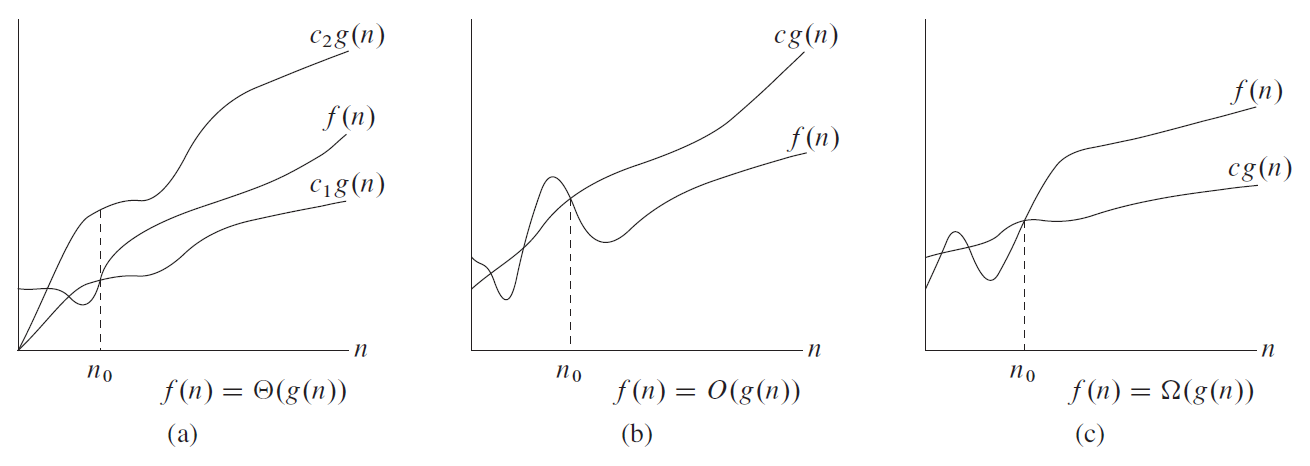
\includegraphics[width=\linewidth]{figuras/big-o}
  \caption{Interpretación gráfica de la notación asintótica. La notación \(f=O(g)\) implica que \(g\) es una cota superior para \(f\); esto es, \(g\) crece más rápido que \(f\) a partir de cierto valor de \(n\).}
\end{marginfigure}

\begin{marginfigure}
  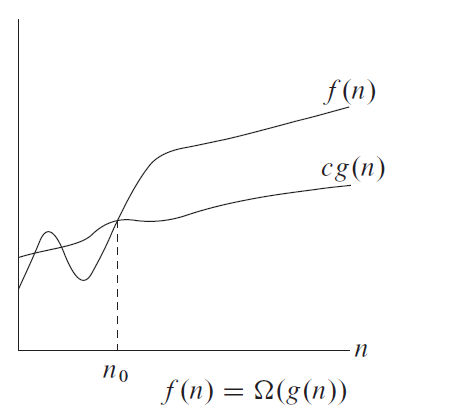
\includegraphics[width=\linewidth]{figuras/big-omega}
  \caption{La notación \(f=\Omega(g)\) implica que \(g\) es una cota inferior para \(f\); esto es, \(g\) crece más lento que \(f\) a partir de cierto valor de \(n\).}
\end{marginfigure}

\begin{marginfigure}
  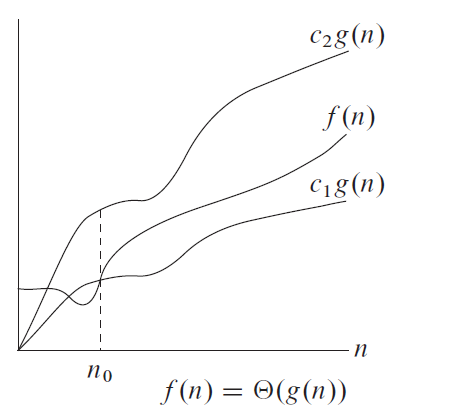
\includegraphics[width=\linewidth]{figuras/big-theta}
  \caption{La notación \(f=\Theta(g)\) implica que \(g\) acota a \(f\) por arriba y por abajo.}
\end{marginfigure}

Sea \(n\in\mathbb{N}\) y sean \(f:\mathbb{N}\to\mathbb{R}\) y \(g:\mathbb{N}\to\mathbb{R}\) dos funciones \textbf{asintóticamente no-negativas}; esto es, siempre se tiene que \(f(n)\geq 0\) y \(g(n)\geq 0\) a partir de algún valor determinado de \(n\). 

\begin{defn}[\textbf{O-grande}]
  Denotado como \(O(g)\), es el conjunto de todas aquellas funciones \(f\) para las cuales existen dos constantes, \(c\in\mathbb{R}^+\) y \(n_0\in\mathbb{N}\), tales que \(0\leq f(n)\leq cg(n)\) para toda \(n\leq n_0\).
\end{defn}

\begin{defn}[\(\boldsymbol{\Omega}\)\textbf{-grande}]
  Denotado como \(\Omega(g)\), es el conjunto de todas aquellas funciones para las cuales existen dos constantes, \(c\) y \(n_0\), tales que \(0\leq cg(n)\leq f(n)\) para toda \(n\geq n_0\).
\end{defn}

\begin{defn}[\(\boldsymbol{\Theta}\)\textbf{-grande}]
  Denotado como \(\Theta(g)\), es el conjunto de todas aquellas funciones para las cuales existen tres constantes, \(c_1,c_2\in\mathbb{R}^+\) y \(n_0\), tales que \(0\leq c_1 g(n)\leq f(n)\leq c_2 g(n)\) para toda \(n\geq n_0\).
\end{defn}

\begin{prop}
  Se tiene q. \(f=\Theta(g)\) si y solo si \(f=O(g)\) y \(f=\Omega(g)\).
\end{prop}

\begin{defn}[\textbf{o-chica}]
  Denotado como \(o(g)\), es el conjunto de todas aquellas funciones \(f\) para las cuales se cumple que, para toda constante \(c\), existe una constante \(n_0\) tal que \(0\leq f(n)<cg(n)\) para toda \(n\leq n_0\).
\end{defn}

\begin{defn}[\(\boldsymbol{\omega}\)\textbf{-chica}]
  Denotado como \(\omega(g)\), es el conjunto de todas aquellas funciones \(f\) para las cuales se cumple que, para toda constante \(c\), existe una constante \(n_0\) tal que \(0\leq cg(n)<f(n)\) para toda \(n\geq n_0\).
\end{defn}

\begin{prop}
  Si \(f=o(g)\), entonces \(f=O(g)\).
\end{prop}

\begin{prop}
  Si \(f=\omega(g)\), entonces \(f=\Omega(g)\).
\end{prop}

\begin{prop}
  Se tiene que
  \[
    \text{si }\lim_{n\to\infty}\dfrac{f(n)}{g(n)}=\begin{cases}
    0 & \text{entonces }f=o(g)\\
    \infty & \text{entonces }f=\omega(g)\\
    1 & \text{entonces }f=\Theta(g).
    \end{cases}
  \]
\end{prop}

\newpage
\section{Comparación de funciones por medio de la notación asintótica}

La notación asintótica se puede utilizar para comparar dos funciones y decidir cuál crece más rápido.

\begin{table}
  \label{tab:func-comp}
  \caption{Operaciones de comparación de los números reales y su funcionamiento análogo en la notación asintótica.}
  \centering
  \begin{tabular}{cc}
    \toprule 
      Números reales & Notación asintótica\tabularnewline
    \midrule
      \(a\leq b\) & \(f=O(g)\)\tabularnewline
      \(a\ge b\) & \(f=\Omega(g)\)\tabularnewline
      \(a=b\) & \(f=\Theta(g)\)\tabularnewline
      \(a<b\) & \(f=o(g)\)\tabularnewline
      \(a>b\) & \(f=\omega(g)\)\tabularnewline
    \bottomrule
  \end{tabular}
\end{table}

\paragraph{Transitividad} 
  Sea \(h:\mathbb{N}\to\mathbb{R}\) una función asintóticamente positiva.
  \begin{itemize}
    \item Si \(f=O(g)\) y \(g=O(h)\), entonces \(f=O(h)\).
    \item Si \(f=\Omega(g)\) y \(g=\Omega(h)\), entonces \(f=\Omega(h)\).
    \item Si \(f=\Theta(g)\) y \(g=\Theta(h)\), entonces \(f=\Theta(h)\).
    \item Si \(f=o(g)\) y \(g=o(h)\), entonces \(f=o(h)\).
    \item Si \(f=\omega(g)\) y \(g=\omega(h)\), entonces \(f=\omega(h)\).
  \end{itemize}

\paragraph{Reflexividad} 
  Se tiene que \(f=\Theta(f)\), \(f=O(f)\) y \(f=\Omega(f)\). 
  Esto se cumple porque \(f(n)=f(n)\) para toda \(n\).

\paragraph{Simetría y simetría traspuesta}
  \begin{itemize}
    \item \(f=\Theta(g)\) si y sólo si \(g=\Theta(f)\)
    \item \(f=O(g)\) si y sólo si \(g=\Omega(f)\).
    \item \(f=o(g)\) si y sólo si \(g=\omega(f)\).
  \end{itemize}

\paragraph{Carencia de tricotomía} 
  La tricotomía es la propiedad de los números reales donde, dados dos números, \(a\) y \(b\), siempre se cumple necesariamente una de las sig. posibilidades: \(a<b\), \(a=b\) o \(a>b\).
  Puede llegar a ocurrir que no se cumple que \(f=O(g)\) ni que \(f=\Omega(g)\).
  P. ej., el comportamiento asintótico de las funciones \(f(n)=n\) y \(g(n)=n^{1+\sin{n}}\) no se puede comparar porque el exponente \(1+\sin{n}\) oscila entre 0 y 2, tomando todos los valores intermedios y, como consecuencia, ninguna función consistentemente acota a la otra.

\marginnote[-14\baselineskip]{%
  Cabe mencionar que, dado que \(\Theta\)-grande posee las propiedades de reflexividad, transitividad y simetría, este conjunto es, de hecho, una \textbf{relación de equivalencia}.
}

\newpage
\section{Ordenes de crecimiento comúnes}

Listados de aquél que crece más lento al que crece más rápido.

\begin{enumerate}
  \begin{multicols}{2}
    \item \emph{Constantes}: \(O(1)\)
    \item \emph{Logarítmicos}: \(O(\log n)\)
    \item \emph{Radicales}: \(O(\sqrt{n})\)
    \item \emph{Lineales}: \(O(n)\)
    \item \emph{Súper lineales}: \(O(n\log n)\)
    \item \emph{Cuadráticos}: \(O(n^{2})\)
    \item \emph{Cúbicos}: \(O(n^{3})\)
    \item \emph{Exponenciales}: \(O(2^{n})\)
    \item \emph{Factoriales}: \(O(n!)\)
  \end{multicols}
\end{enumerate}

No se debe confiar ciegamente en la lista anterior, ya que la notación asintótica puede ocultar constantes muy grandes y dejar una impresión equivocada del orden de crecimiento de una función comparada con otra.
P. ej., \(f(n)=10^{100}n=O(n)\) y \(g(n)=10n\cdot\log n=O(n\log n)\). 
A pesar de que la notación asintótica indica que \(g\) crece más rápido que \(f\), en realidad se trata de lo opuesto porque la constante \(10^{100}\) supera por mucho el orden de crecimiento de \(g\)

\section{Operaciones aritméticas con la notación asintótica}

\paragraph{Adición}
  \[
  \begin{aligned}
      O(f)+O(g) &= O(\max\{f,g\})\\
      \Omega(f)+\Omega(g) &= \Omega(\max\{f,g\})\\
      \Theta(f)+\Theta(g) &= \Theta(\max\{f,g\})
  \end{aligned}
  \qquad
  \begin{aligned}
      o(f)+o(g) &= o(\max\{f,g\})\\
      \omega(f)+\omega(g) &= \omega(\max\{f,g\})
  \end{aligned}
  \]

\paragraph{Multiplicación}
  \[
  \begin{aligned}
      O(cf) &= O(f)\\
      \Omega(cf) &= \Omega(f)\\
      \Theta(cf) &= \Theta(f)
  \end{aligned}
  \qquad
  \begin{aligned}
      o(cf) &= o(f)\\
      \omega(cf) &= \omega(f)
  \end{aligned}
  \]

  \[
  \begin{aligned}
      O(f)\cdot O(g) &= O(f\cdot g)\\
      \Omega(f)\cdot\Omega(g) &= \Omega(f\cdot g)\\
      \Theta(f)\cdot\Theta(g) &= \Theta(f\cdot g)
  \end{aligned}
  \qquad
  \begin{aligned}
      o(f)\cdot o(g) &= o(f\cdot g)\\
      \omega(f)\cdot\omega(g) &= \omega(f\cdot g)
  \end{aligned}
  \]

\marginnote[-2\baselineskip]{%
  \textbf{Literatura consultada}: \textcite{cormen_2009}, pp. 43-52; \textcite{skiena_2012} pp. 34-41.
}

  % \chapter{Relaciones de Recurrencia}

Una \emph{relación de recurrencia} (o, simplemente, \emph{recurrencia})
es una función expresada en términos de sí misma, pero con una entrada
más pequeña. Las recurrencias se presentan al analizar la
eficiencia de algoritmos de tipo \emph{divide y vencerás}. La \emph{forma
cerrada} de una recurrencia es una función equivalente, pero expresada
sin recursividad. \emph{Resolver} una recurrencia implica encontrar
su forma cerrada.

En el contexto de los algoritmos divide y vencerás, las recurrencias
suelen tener la sig. forma general: 

\[
    T(n)=\begin{cases}
        \sum_{i=1}^{p}T(n_{i})+f(n) & \text{para }n>b\\
        g(n) & \text{en caso contrario}
    \end{cases}
\]
donde

\begin{itemize}
    \item $b\in\mathbb{N}$ es la condición de paro (boundary condition); esto
    es, el valor que debe tener $n$ para entrar al caso base, 
    \item $g:\mathbb{N}\to\mathbb{N}$ es el tiempo de ejecución del caso base, 
    \item $p\in\mathbb{N}$ es la cantidad de subproblemas en las que se dividió
    la entrada, 
    \item $n_{i}\in\mathbb{N}$, tal que $n_{i}<n$, es el tamaño de la entrada
    para el subproblema $i$, 
    \item $f:\mathbb{N}\to\mathbb{N}$ es el tiempo de ejecución para dividir
    la entrada en, y/o combinar las soluciones de los, $p$ subproblemas 
\end{itemize}
La función $g$ suele omitirse cuando es constante. 

A continuación se presentan tres métodos diferentes para resolver
recurrencias.

\section{El método maestro}

El método maestro consiste simplemente en aplicar el sig. teorema.

\begin{thm}[Teorema maestro]
    Sean $a,n\in\mathbb{N}$ y $b\in\mathbb{R}$, donde $a$ y $b$ son
    constantes y $b>1$. Sea $f:\mathbb{N}\to\mathbb{N}$ una función
    asintóticamente positiva y sea $c=\log_{b}a$. Si $T:\mathbb{N}\to\mathbb{N}$
    es una recurrencia de la forma $T(n)=aT(n/b)+f(n)$, entonces se puede
    resolver de las sig. maneras:
    \begin{enumerate}
        \item Si $f=O(n^{c-\varepsilon})$ para alguna constante real $\varepsilon>0$,
        entonces $T=\Theta(n^{c})$.
        \item Si $f=\Theta(n^{c})$, entonces $T=\Theta(n^{c}\log n)$.
        \item Si $f=\Omega(n^{c+\varepsilon})$ y si, además, $af(n/b)\leq kf(n)$
        para alguna constante real $k<1$ y para todo valor de $n$ pasado
        algún umbral, entonces $T=\Theta(f)$.
    \end{enumerate}
\end{thm}

\begin{rem}
    Para el Teorema Maestro, el término $n/b$ también se puede interpretar
    como $\lceil n/b\rceil$ o $\lfloor n/b\rfloor$.
\end{rem}

La principal desventaja del Teorema Maestro es que no puede aplicarse
a cualquier tipo de recurrencia.

\section{El método del árbol recursivo}

El método del árbol recursivo es un método gráfico e informal que
consiste de construir un árbol donde cada sub-árbol representa el
tiempo requerido para resolver un subproblema en la recurrencia. Al
sumar el tiempo total de cada nivel del árbol se obtiene la forma
cerrada. 

Antes de estudiar el método en sí, es importante recordar las sig.
propiedades de los árboles $k$-arios.

\begin{prop}
    Sea $k\in\mathbb{N}_{0}$ y $n\in\mathbb{N}$. La altura de un árbol
    $k$-ario de $n$ nodos se calcula como $\lfloor\log_{k}n\rfloor+1$.
\end{prop}

\begin{prop}
    Sea $i\in\mathbb{N}_{0}$. Suponiendo que la raíz de un árbol $k$-ario
    completo se encuentra en el nivel 0, la cantidad de nodos en el nivel
    $i$, se calcula como $k^{i}$.
\end{prop}

El método del árbol recursivo consiste de los sig. pasos:

\begin{enumerate}
    \item Desglozar la recurrencia en un árbol de tal forma que la raíz represente
    el tiempo requerido para combinar y/o dividir el problema original,
    cada nodo interno represente el tiempo requerido para combinar y/o
    dividir un subproblema y cada hoja represente el tiempo requerido
    por el caso base. 
    \item Calcular la altura del árbol.
    \item Calcular la cantidad de hojas.
    \item Para cada nivel, sumar el tiempo de ejecución de todos sus nodos. 
    \item Sumar el tiempo de ejecución de todos los niveles para obtener la
    forma cerrada.
\end{enumerate}

\section{El método de sustitución}

El método de sustitución es un método formal que consiste en resolver
una recurrencia por inducción matemática. Específicamente, este método
consiste de los sig. pasos:

\begin{enumerate}
    \item Proponer una cota asintótica como la solución tentativa
    para la recurrencia.
    \item Utilizar inducción matemática para demostrar que la cota propuesta
    es correcta y para encontrar las constantes de dicha cota.
\end{enumerate}

Este método se puede utilizar para calcular tanto una cota superior
como una inferior. A continuación se presentan algunas consideraciones
y consejos que se deben tener en cuenta al trabajar con este método. 

\begin{itemize}
    \item Para proponer una buena solución tentativa:
    \begin{itemize}
        \item Se puede utilizar el método del árbol recursivo para obtener una solución
        tentativa y después utilizar el método de sustitución para demostrar
        que dicha solución es correcta o para ajustar la cota.
        \item Si la recurrencia tiene una forma similar a alguna cuya solución ya
        se conoce, se puede proponer esa solución como tentativa.
        \item Se pueden proponer dos cotas holgadas, una inferior y una superior,
        y ajustarlas gradualmente hasta que converjan en la solución correcta. 
    \end{itemize}
    \item Diferencias con la inducción matemática:
    \begin{itemize}
        \item El caso base se realiza hasta el último.
        \item La hipótesis inductiva consiste de suponer que la cota se cumple para
        $T(n_{i})$.
        \item El paso inductivo consiste en sustituir $T(n_{i})$, en la recurrencia
        original, por la forma exacta de la cota de la hipótesis inductiva.
        Este paso da origen al nombre del método.
    \end{itemize}
    \item Se debe demostrar algebraicamente que la cota propuesta se cumple
    de forma exacta. Es incorrecto aplicar la notación asintótica en el
    paso inductivo para deshacerse de constantes o términos problemáticos.
    \item Cuando la cota popuesta es lo más ajustada posible, pero aún así la
    inducción no converge, en lugar de proponer una cota más holgada,
    se puede proponer una nueva hipótesis inductiva cuya única diferencia
    con la anterior es que se le restan los términos de menor grado.
\end{itemize}

\section{Cambio de variable}

En ocasiones, se puede aplicar álgebra para transformar una recurrencia
en alguna otra cuya solución ya se conozca, eliminando
la necesidad de recurrir a cualquiera de los métodos anteriores.

\section*{Notas bibliográficas}

En las págs. 97-106 del libro de \textcite{cormen_introduction_2009} se
proporciona la demostración del Teorema Maestro. 

En las págs. 112 y 113
se proporcionan referencias a otros métodos que existen para resolver 
diferentes tipos
de recurrencias. Uno de los cuáles es el método de Akra-Bazzi, el cual
es una generalización del Teorema Maestro que admite variables contínuas
y permite resolver recurrencias donde los subproblemas varían substancialmente
de tamaño. El método de \textcite{drmota_master_2013} es una extensión
del método de Akra-Bazzi para trabajar con variables discretas. 

\begin{itemize}
    \item \textcite{cormen_introduction_2009}, págs. 83-106 y 112-113.
    \item \textcite{akra_solution_1998}.
    \item \textcite{drmota_master_2013}.
    \item \textcite{goodrich_algorithm_2001}, pág. 12.
\end{itemize}

  
  \appendix
    % \chapter{Redacción Matemática}

A diferencia de otras áreas de la ciencia, el estudio de las matemáticas
no se dedica a la recolección de evidencia física, sino a la manipulación
de conceptos abstractos y la presentación de argumentos lógicos. Es
por ello que es de suma importancia desarrollar la habilidad de buena
redacción en esta área (y, por extensión, en las ciencias de la 
computación). A continuación se proporcionan algunos consejos sobre cómo 
redactar correctamente ``trabajos matemáticos''
(i.e. artículos, reportes, ensayos, tareas, etc.).

\section{Organización del contenido}

Antes de comenzar a elaborar un trabajo escrito, es recomendable preparar
lo sig.:

\begin{itemize}
    \item Los antecedentes y la motivación del trabajo.
    \item Las definiciones y la notación a ser utilizadas.
    \item Los ejemplos a ser incluidos.
    \item Los resultados a ser presentados con sus demostraciones correspondientes
    (posiblemente en borrador). 
    \item Referencias a otros resultados que se pretenden utilizar.
    \item El orden en que todo lo anterior será presentado.
\end{itemize}

Si se prepara de antemano esta información, es más fácil escribir
el trabajo, pues sólo se requiere seguir el plan trazado.

\section{Uso apropiado de símbolos}

\begin{itemize}
    \item Nunca se debe iniciar una oración con un símbolo o una ecuación; es 
    preferible iniciar con un sustantivo seguido del símbolo que se pretende utilizar.
    Por ejemplo, en lugar de escribir:
    
    \[
        \pi\text{ es un número irracional.}
    \]
        
    es preferible escribir:
    
    \[
        \text{La constante }\pi\text{ es un número irracional.}
    \]
    
    \item De ser posible, se deben utilizar palabras en lugar de comas para separar
    aquellos símbolos que no conformen una lista. Por ejemplo, en lugar
    de escribir:
    
    \[
        \text{Al igual que }\pi\text{, }e\text{ es un número irracional.}
    \]
        
    es preferible escribir:
    
    \[
        \text{Al igual que }\pi\text{, la constante }e\text{ es un número irracional.}
    \]

    \item Se debe evitar el uso de símbolos lógicos (como $\forall$,
    $\exists$, $\Rightarrow$, i.a.) si el tema que se está tratando no
    pertenece al área de la lógica. Estos símbolos se utilizan comúnmente 
    para sustituir frases matemáticas de uso frecuente. Esta práctica es 
    aceptable si se está trabajando en un borrador o se están tomando apuntes. 
    Sin embargo, cuando se trata de trabajos formales o profesionales, 
    esta práctica debe evitarse.

    \item Se debe evitar el uso de las abreviaciones ``i.e.'' y ``e.g.''
    si se están utilizando símbolos parecidos. Si no se tiene cuidado de cómo 
    se utilizan, pueden hacer confusa la redacción. Por ejemplo, 
    en lugar de escribir ``las expresiones
    $\sqrt{-1}$ y $\lim_{n\to\infty}\left(1+1/n\right)^{n}$ no son números
    racionales; i.e. $i$ y $e$ son irracionales'' es preferible escribir:
    ``las expresiones $\sqrt{-1}$ y $\lim_{n\to\infty}\left(1+1/n\right)^{n}$
    no son números racionales; esto es, las constantes $i$ y $e$ son
    irracionales''.

    \item Todo número utilizado como un cuantificador se debe escribir con letra.
    Por ejemplo, es preferible escribir:
    
    \[
        \text{Hay exactamente dos grupos de orden 4.}
    \]
    \[
        \text{Cincuenta millones de personas no pueden estar equivocadas.}
    \]
    \[
        \text{Hay un millón de enteros positivos menores a 1,000,001.}
    \]
    
    \item No se deben mezclar símbolos con palabras en una misma oración. Por
    ejemplo, en lugar de escribir:
    
    \[
        \text{Todo entero }>1\text{ es primo o compuesto.}
    \]
    
    es preferible escribir:
    
    \[
        \text{Todo entero que mayor a 1 es primo o compuesto.}
    \]

    Otro ejemplo; aunque la sig. oración puede sonar correcta, está mal
    redactada:
    
    \[
        \text{Como }(x-2)(x-3)=0\text{, se tiene que }x=2\text{ o }3.
    \]
    
    En este caso, es preferible escribir:
    
    \[
        \text{Como }(x-2)(x-3)=0\text{, se tiene que }x=2\text{ o }x=3.
    \]

    \item No se deben introducir símbolos si no se van a utilizar. Por ejemplo,
    en la oración ``toda función biyectiva $f$ tiene una inversa'',
    si el símbolo $f$ no se vuelve a utilizar en el texto, entonces
    es preferible omitirlo. 

    \item No se deben usar símbolos sin primero haberlos introducido. Por ejemplo,
    si se tiene la expresión $n=2k+1$ y esta es la primera vez que aparece
    el símbolo $k$, entonces es preferible redactar esta expresión como:
    
    \[
        \text{Sea }k\text{ un entero, se tiene que }n=2k+1.
    \]
    \[
        \text{Se tiene que }n=2k+1\text{, donde }k\text{ es un entero.}
    \]
    
    \item Se deben seguir convenciones bien establecidas sobre el uso de
    algunos símbolos. Hay convenciones que se vienen utilizando en la
    literatura desde hace mucho tiempo y, debido a ello, uno debe apegarse
    a ellas. Algunas de estas convenciones son:

    \begin{itemize}
        \item Las letras $a$, $b$ y $c$ representan constantes. 
        \item Las letras $x$, $y$ y $z$ representan variables. 
        \item Las letras $m$ y $n$ representan enteros. 
        \item Las letras $i$ y $j$ representan índices.
        \item Las letras $f$, $g$ y $h$ representan funciones. 
        \item Las letras $u$, $v$ y $w$ representan vectores. 
        \item Las letras mayúsculas representan conjuntos o matrices.
    \end{itemize}
    
    \item Se deben utilizar parejas apropiadas de símbolos. Por ejemplo, usar
    $a$ junto con $b$ o utilizar $p$ junto con $q$, etc.

\end{itemize}

\section{Escritura de expresiones algebraicas}

Como regla general, si una expresión algebraica es relativamente corta,
entonces se puede escribir en el mismo renglón que el resto del texto.
De lo contrario, es preferible dedicarles su propio renglón, para evitar 
que una expresión larga tenga que separarse en dos renglones. 
Por otro lado, en el caso de manipulaciones algebraicas extensas, es 
recomendable saltar de renglón cada vez que se introduce
un símbolo de comparación. También es recomendable alinear todos los
símbolos de comparación en una misma columna. Por último, en aquellos
casos donde sea inevitable separar una expresión en dos renglones, es 
preferible hacerlo de tal forma que el primer renglón termine con un 
símbolo de operación y el siguiente comience con un término. De esta forma,
queda claro para el lector que la expresión en el primer renglón
está incompleta y continúa en el siguiente. 

\section{Uso apropiado de frases comunes}

\begin{itemize}

    \item Se debe utilizar el artículo ``se'' en lugar de los pronombres ``yo'',
    ``nosotros'' y ``uno''. Usar ``yo'' se considera egocéntrico,
    a menos que se hable sobre alguna experiencia personal. Usar ``nosotros''
    es adecuado, pero se corre el riesgo de sonar demasiado informal. El
    uso de ``uno'' es posible e incluso preferible en algunos casos,
    pero en otros puede ser incorrecto. El uso del artículo ``se'', seguido
    de un verbo conjugado adecuadamente, es una forma de redacción 
    muy flexible y por eso se recomienda su uso sobre los pronombres. 
    Por ejemplo, considere las sig. oraciones y compare cuál suena más apropiado:
    
    \begin{itemize}
        \item Ahora demostraré que $n$ es par.
        \item Ahora demostraremos que $n$ es par.
        \item Ahora uno demostrará que $n$ es par.
        \item Ahora se demostrará que $n$ es par.
    \end{itemize}
    
    \item Se debe evitar el uso de palabras como ``claramente'', ``obviamente'',
    ``trivialmente'', i.a. Al usar estas frases, 
    se corre el riesgo de que lo que se describe a continuación no quede 
    absolutamente claro para el lector, en cuyo caso se dejaría una mala impresión
    sobre el dominio del tema o una mala experiencia de lectura.
    
    \item Se debe tener cuidado de cómo se utilizan las frases ``para cualquier'',
    ``para algún'' y ``para todo''. Estas frases se consideran como
    equivalentes en la redacción matemática pero, si no se tiene
    cuidado del contexto en que se usan, pueden resultar en ambigüedades.
    Por ejemplo, considere la sig. oración: ``Se dice que el conjunto
    $S$ satisface la propiedad $P$ si $P$ se satisface para cualquier
    elemento $s\in S$''. En este caso, queda ambigüo si la propiedad
    $P$ se debe cumplir para todos los elementos de $S$ o solamente
    para uno. En situaciones como esta, es preferible evitar completamente
    la frase ``para cualquier'' en favor de una redacción más explícita;
    e.g. utilizando frases como ``para todo/cada'', ``para algún''
    o ``para al menos uno''.
    
    \item Es incorrecto utilizar la palabra ``como'' en conjunto con ``entonces''.
    Por ejemplo, en lugar de escribir:
    
    \[
        \text{Como }n^{2}\text{ es par, entonces }n\text{ también es par.}
    \]
    
    es preferible escribir cualquiera de estas:

    \[
        \text{Si }n^{2}\text{ es par, entonces }n\text{ también es par.}
    \]
    \[
        \text{Como }n^{2}\text{ es par, se tiene que }n\text{ también es par.}
    \]
    \[
        \text{Como }n^{2}\text{ es par, }n\text{ también es par.}
    \]
    
    \item No se debe utilizar en cantidades abusivas frases como ``por lo tanto'',
    ``lo que implica'', ``como consecuencia'', etc. El propósito de
    estas frases es encadenar varios razonamientos para formar un
    argumento lógico. Utilizar la misma frase de forma repetitiva
    puede volverse muy tedioso para el lector. Debido a ello, se recomienda 
    utilizar una variedad más amplia de frases y, por lo menos, se debe evitar 
    utilizar la misma frase dos veces seguidas. Naturalmente, esto requiere de 
    creatividad y práctica.

\end{itemize}

\section{Consejos generales}

\begin{itemize}
    \item Se deben escribir oraciones completas y que sean gramatical y ortográficamente
    correctas. Se sugiere conjugar igual todos los verbos de una misma oración y utilizar
    conjugaciones simples siempre que sea posible. 
    \item La escritura es un proceso iterativo; rara vez se puede escribir algo
    correctamente en el primer intento. Es por ello que se recomienda
    releer \emph{desde el principio} el trabajo que se está escribiendo
    cada vez que se le hace alguna corrección. También es recomendable
    dejar descansar el escrito unos días antes de volver a revisarlo. 
    \item A la hora de escribir, se debe considerar la audiencia para la que
    se está escribiendo; esto es, se debe elegir el vocabulario y estilo
    de redacción adecuados para ella y se debe considerar su conocimiento
    previo al decidir cuánta información incluir y cuánta omitir. 
    \item Nunca se debe entregar o publicar un trabajo escrito sin antes permitir
    que alguien más lo lea y proporcione retroalimentación. Además, toda
    corrección realizada al escrito debe ser verificada por la misma persona
    que sugirió dicha corrección.
\end{itemize}

\section*{Notas bibliográficas}

\begin{itemize}
    \item \textcite{chartrand_mathematical_2012}, págs. 1-13.
\end{itemize}
%% mover a matematicas discretas
    \chapter{La potencia}

Sea \(x\in\mathbb{R}\) distinto de cero y denominado \emph{base} y sea \(n\in\mathbb{N}\) denominado \emph{exponente}. 
La \emph{n-ésima potencia} de \(x\), denotada como \(x^n\), es el producto de \(n\) bases \(x\); esto es, \(x^n\triangleq x\cdot x\cdot\dots(n\text{ veces})\).

\section{Leyes de los exponentes}

Sean \(x,y\in\mathbb{R}\) distintos de cero y sean \(m,n\in\mathbb{N}\).
Se tienen las sig. identidades:
\begin{enumerate}
  \begin{multicols}{3}
    \item \(x^{0}\triangleq1\)
    \item \(x^{1}\triangleq x\)
    \item \(x^{-1}\triangleq1/x\)
    \item \(x^{m/n}\triangleq\sqrt[n]{x^{m}}\)
    \item \(x^{m}x^{n}=x^{m+n}\)
    \item \(x^{m}/x^{n}=x^{m-n}\)
    \item \((x^{m})^{n}=x^{mn}\)
    \item \((xy)^{n}=x^{n}y^{n}\)
    \item \((x/y)^{n}=x^{n}/y^{n}\)
  \end{multicols}
\end{enumerate}

Las identidades anteriores se justifican de las sig. manipulaciones algebraicas:

\begin{flalign}\tag{5}
  x^mx^n &= x\cdot x\cdot\dots (m\text{ veces})\cdot x\cdot x\dots (n\text{ veces}) &&\\
  &= x^{m+n}\nonumber
\end{flalign}

\begin{flalign}\tag{6}
  \text{\textit{Caso 1}} &: \text{ Si }m>n\text{, entonces} \nonumber&&\\
  x^m/x^n &= \dfrac{x\cdot x\cdot\dots (m\text{ veces})}{x\cdot x\cdot\dots (n\text{ veces})} \nonumber&&\\
  &= 1\cdot 1\cdot\dots(n\text{ veces})\cdot x\cdot x\cdot\dots(m-n\text{ veces}) \nonumber&&\\
  &=x^{m-n} \nonumber&&\\
  \text{\textit{Caso 2}} &: \text{ Si }m=n\text{, entonces} \nonumber&&\\
  x^m/x^n &=1\cdot 1\cdot\dots (m=n\text{ veces}) \nonumber&&\\
  &=x^0 \nonumber&&\\
  &=x^{m-n}\nonumber&&\\
  \text{\textit{Caso 3}} &: \text{ Si }m<n\text{, entonces} \nonumber&&\\
  x^m/x^n &=1\cdot 1\cdot\dots(m\text{ veces})\cdot 1/x\cdot 1/x\cdot\dots(n-m\text{ veces}) \nonumber&&\\
  &=1/x^{n-m} \nonumber&&\\
  &=x^{m-n} \nonumber
\end{flalign}

\begin{flalign}\tag{7}
  (x^m)^n &= [x\cdot x\cdot\dots (m\text{ veces})]\cdot[x\cdot x\cdot\dots (m\text{ veces})]\dots[n\text{ veces}] &&\\
  &= x^{mn}\nonumber
\end{flalign}

\begin{flalign}\tag{8}
  (xy)^n &= xy\cdot xy\cdot\dots (n\text{ veces}) &&\\
  &= x\cdot x\cdot\dots (n\text{ veces})\cdot y\cdot y\cdot\dots (n\text{ veces}) \nonumber&&\\
  &= x^ny^n\nonumber
\end{flalign}

\begin{flalign}\tag{9}
  (x/y)^n &= \dfrac{x}{y}\cdot\dfrac{x}{y}\cdot\dots (n\text{ veces}) &&\\
  &= x^n/y^n\nonumber
\end{flalign}

    \chapter{El logaritmo}

Sea \(x\in\mathbb{R}\) mayor a cero y denominado \emph{argumento} y sea \(b\in\mathbb{R}\) distinto de 1 y denominado \emph{base}.
El \emph{logaritmo} de \(x\) con respecto a \(b\), denotado como \(\log_{b}x\), es la potencia a la que hay que elevar \(b\) para obtener \(x\) como resultado; esto es, \(y=\log_{b}x\) si y sólo si \(b^{y}=x\), donde \(y\in\mathbb{R}\).

\begin{table}[h]
  \caption{Diferentes tipos de logaritmos, su base y su notación correspondiente.}
  \begin{center}
    \begin{tabular}{ccc}
      \toprule
      Tipo de logaritmo & Base & Notación \\
      \midrule
      Decimal & 10 & \(\log{x}\) \\
      Natural & \(e\) & \(\ln{x}\) \\
      Binario & 2 & \(\lg{x}\) \\
      \bottomrule
    \end{tabular}
  \end{center}
\end{table}

\begin{prop}
  La base de un logaritmo no puede ser 0 ni 1.
\end{prop}
  
Debido a que \(0^x=0\) para toda \(x>0\) y debido a que \(1^x=1\) para toda \(x\), los logaritmos con base 0 y 1 no tienen una solución definida.

\begin{prop}
  La base de un logaritmo no puede ser negativa.
\end{prop}

De lo contrario, dependiendo del argumento del logaritmo, la solución podría ser un número complejo.

\begin{prop}
  El argumento de un logaritmo no puede ser negativo.
\end{prop}

Debido a que todo número positivo elevado a cualquier potencia siempre resulta en un número positivo, el logaritmo (con base positiva) de un número negativo no tendría solución.

\section{Leyes de los logaritmos}

Sean \(b,v,x,y\in\mathbb{R}\), donde los valores \(x\) y \(y\) son mayores a cero y los valores \(b\) y \(v\) son distintos de 1. Se tienen las sig. identidades:

\marginnote[1\baselineskip]{La identidad 7 se conoce como la ley de cambio de base. Esta ley implica que \(\log_v{x}=\log_v{b}\cdot\log_b{x}\); esto es, para cambiar la base de un logaritmo, basta con multiplicarlo por un factor constante. Debido a esto, no importa la base de un logaritmo, su comportamiento asintótico siempre será el mismo y es por esta razón que la base del logaritmo suele omitirse al utilizar la notación asintótica.}

\begin{enumerate}
  \begin{multicols}{2}
    \item \(\log_b{1}=0\)
    \item \(\log_b{b}=1\)
    \item \(\log_b(xy)=\log_b{x}+\log_b{y}\)
    \item \(\log_b(x/y)=\log_b{x}-\log_b{y}\)
    \item \(\log_bx^y=y\log_b{x}\)
    \item \(\log_b\sqrt[y]{x}=1/y\cdot\log_b{x}\)
    \item \(\log_b{x}=\log_v{x}/\log_v{b}\)
    \item \(\log_b{x}=1/\log_x{b}\), si \(x\neq 1\)
    \item \(x^{\log_b{y}}=y^{\log_b{x}}\)
  \end{multicols}
\end{enumerate}

Las identidades anteriores se justifican de las manipulaciones algebraicas que se presentan a continuación. Considérese que \(p,q\in\mathbb{R}\) tales que \(x=b^p\) y \(y=b^q\), lo que implica que \(p=\log_b{x}\) \& \(q=\log_b{y}\) (por la definición del logaritmo):
\begin{flalign}
  \text{Es consecuencia directa del hecho que } b^0=1\text{ para cualquier }b.
\end{flalign}
\begin{flalign}
  \text{Es consecuencia directa del hecho que } b^1=b\text{ para cualquier }b.
\end{flalign}
\begin{align}
  xy &= b^pb^q &&\\
  xy &= b^{p+q} \nonumber&&\\
  \log_b(xy) &= p+q \nonumber&&\\
  \log_b(xy) &= \log_b{x}+\log_b{y} \nonumber
\end{align}
\begin{align}
  x/y &= b^p/b^q &&\\
  x/y &= b^{p-q} \nonumber&&\\
  \log_b(x/y) &= p-q \nonumber&&\\
  \log_b(x/y) &= \log_b{x}-\log_b{y} \nonumber
\end{align}
\begin{align}
  x &= b^p &&\\
  x^y &= (b^p)^y \nonumber&&\\
  x^y &= b^{py} \nonumber&&\\
  \log_b{x^y} &= py \nonumber&&\\
  \log_b{x^y} &= y\log_b{x} \nonumber
\end{align}
\begin{align}
  x &= b^p &&\\
  \sqrt[y]{x} &= \sqrt[y]{b^p} \nonumber&&\\
  \sqrt[y]{x} &= b^{p/y} \nonumber&&\\
  \log_b \sqrt[y]{x} &= p/y \nonumber&&\\
  \log_b \sqrt[y]{x} &= 1/y\cdot \log_b{x} \nonumber
\end{align}
\begin{align}
  b^p &= x &\\
  \log_v{b^p} &= \log_v{x} \nonumber&&\\
  p\log_v{b} &= \log_v{x} \nonumber&&\\
  p &= \dfrac{\log_v{x}}{\log_v{b}} \nonumber&&\\
  \log_b{x} &= \log_v{x}/\log_v{b} \nonumber
\end{align}
\begin{align}
  \log_b{x} &= \dfrac{\log_v{x}}{\log_v{b}} &&\\
  \log_b{x} &= \dfrac{\log_x{x}}{\log_x{b}} \nonumber&&\\
  \log_b{x} &= \dfrac{1}{\log_x{b}} \nonumber
\end{align}
\begin{align}
  x^{\log_b{y}}=x^q=(b^p)^q=b^{pq}=(b^q)p=y^p=y^{\log_b{x}}
\end{align}

  
  \printbibliography[heading=bibintoc,title={Literatura consultada}]
\end{document}
